\documentclass{beamer}

\mode<presentation>
{
    %\usetheme{Warsaw}
    \definecolor{links}{HTML}{2A1B81}
    \hypersetup{colorlinks,linkcolor=,urlcolor=links}
    \usetheme{Frankfurt}
    %\usecolortheme{seagull}
    % or ...
    \setbeamercovered{transparent}
    % or whatever (possibly just delete it)
}

\usepackage[english]{babel}
\usepackage[utf8]{inputenc}
\usepackage{times}
\usepackage[T1]{fontenc}
\usepackage{fancyvrb}
\usepackage{listings}
\usepackage{graphicx}
\usepackage{attachfile}
\usepackage{ifthen}

\newboolean{localPieces} %Declaration, defaults to false
\setboolean{localPieces}{false} %Assignment

\title{Advanced Csound}

\author[Gogins]
{Michael Gogins \\ \url{http://michaelgogins.tumblr.com}}

\institute[Irreducible Productions]{Irreducible Productions \\ New York}
\date[NYCEMF 2022]{NYCEMF 2022}

\subject{Computer Music}
\expandafter\def\expandafter\insertshorttitle\expandafter{%
    \insertshorttitle\hfill%
    \insertframenumber\,/\,\inserttotalframenumber}
% This is only inserted into the PDF information catalog. Can be left
% out. 
\begin{document}
\lstset{basicstyle=\ttfamily\tiny,commentstyle=\ttfamily\tiny,tabsize=2,breaklines,fontadjust=true,keepspaces=false,fancyvrb=true,showstringspaces=false,moredelim=[is][\textbf]{\\emph\{}{\}}}

\maketitle

\begin{frame}{Agenda}
\tableofcontents
\end{frame}

\section{Who is this for?}
\begin{frame}{Who is this for?}
\begin{itemize}
\item This workshop is for anyone who uses Csound to \emph{actually make music}.
\item That includes beginners, expert users, and even programmers.
\item I provide examples/exercises that are pre-written to speed things up. You should run them, but you should not have to debug them.
\item The examples are written for macOS, Linux, and Windows, but the ideas also apply to Android and WebAssembly.
\end{itemize}
\end{frame}

\section{What is Csound?}
\begin{frame}{What is Csound?}
\begin{itemize}
\item \emph{Csound is a programmable software sound synthesis system with a runtime compiler.}
\item Csound was written in 1985, so has \emph{more unit generators} than later SWSS such as SuperCollider or Max.
\item Csound runs on desktops, mobile devices, single-board computers, and Web browsers (WebAssembly).
\item Csound has a straightforward "C" API (csound.h).
\item The Csound API has interfaces in C++, Python, Lua, Lisp, and other languages. \emph{You can run Csound inside other languages.}
\item Csound has opcodes for hosting external plugins and even external languages (Python, C++, Lua). \emph{You can run other languages inside Csound.}
\end{itemize}
\end{frame}

\section{Installing Csound}
\begin{frame}{Getting Csound}
Install with brew on macOS, apt on Linux, vcpkg on Windows, or 
google for downloads.
\begin{itemize}
\item Install Csound for your desktop (\url{https://csound.com/download.html}). For the \emph{current} release on
Linux, build from sources
(\url{https://github.com/csound/csound/blob/develop/BUILD.md}).
\item Install the Audacity soundfile editor (\url{https://www.audacityteam.org/download/}).
\item Consider building the Csound external plugins repository (\url{https://github.com/csound/plugins}) from sources and installing it.
\end{itemize}
\end{frame}

\begin{frame}{Configuring}
\begin{itemize}
\item The \texttt{csound} program should be in your environment's \texttt{PATH} variable.
\item For the \texttt{vst4cs opcodes}, we configure Csound to load them from their build or download directories.
\item For the Csound plugins repository, we build them locally and install using \texttt{sudo make install}.
\item Shown for macOS, but the same variables should be set with appropriate values on Linux or Windows.
\end{itemize}
\end{frame}

\begin{lstlisting}
export OPCODE6DIR64="/Users/michaelgogins/Downloads"
export RAWWAVE_PATH="/opt/homebrew/Cellar/stk/4.6.2/share/stk/rawwaves"
\end{lstlisting}

\begin{frame}{M1 Macintosh}
\begin{itemize}
\item Apple's arm64 M1 processor is fantastic, but can create problems of software incompatibility.
\item Some software distributed for Csound is built for x86-amd or x86-64 architecture only, and won't work with software built for arm64 only.
\item Currently, if you have an M1 Mac, CsoundQt and the plugins in the Risset package manager don't work.
\item If you have an \emph{Intel} Mac:
\begin{itemize}
\item Install CsoundQt (\url{http://csoundqt.github.io/pages/install.html}).
\item Install the Risset package manager for Csound plugins (\url{https://github.com/csound-plugins/risset}). 
\end{itemize}
\end{itemize}
\end{frame}

\begin{frame}{Other useful software}
Some of these have their own additional pre-requisites.
\begin{itemize}
\item Python 3.9 (\url{https://www.python.org/downloads/}).
\item ABX comparator (\url{https://github.com/gogins/python-abx}).
\item Faust DSP language (\url{https://github.com/grame-cncm/faust/releases}).
\end{itemize}
\end{frame}

\section{Running Csound}
\begin{frame}{Running Csound}
Csound does not have a built-in code editor or visual patcher like SuperCollider or Max.
\begin{itemize}
\item You can run Csound from the command line.
\item You can run Csound from a general-purpose but customized code editor.
\item You can run Csound from a purpose-built Csound code editor such as CsoundQt.
\item In this workshop, we use any text editor and the command line as the lowest common denominator.
\end{itemize}
\end{frame}

\begin{frame}{Running Csound from the command line}
\begin{example}
Change to the \texttt{exercises/commandline} directory of your workshop directory.
\begin{itemize}
\item Execute \texttt{csound electric-priest.csd} to make sure that Csound runs.  Also make sure that the maximum level at the end is negative so you won't blow out your speakers!
\item Execute \texttt{csound ---devices} to list your system's audio devices.
\item Execute e.g.\  \texttt{csound electric-priest.csd -odac0} to render the piece with real-time audio.
\end{itemize}
\end{example}
\end{frame}

\begin{frame}{Other code editors for Csound}
\begin{itemize}
\item SciTE as customized in csound-extended (\url{https://github.com/gogins/csound-extended/blob/master/playpen/.SciTEUser.properties}).
\item gedit as customized in csound-extended (\url{https://github.com/gogins/csound-extended/blob/master/playpen}).
\item blue (\url{https://blue.kunstmusik.com/}).
\item Cabbage (\url{https://www.cabbageaudio.com/}).
\item Visual Studio Code (\url{https://code.visualstudio.com/}) with
Csound extension (\url{https://github.com/csound/csound-vscode-plugin}).
\end{itemize}
\end{frame}

\begin{frame}{The playpen concept}
\begin{itemize}
\item A "playpen" is where you can play with things and not worry 
about breaking them.
\item In computer music we have an iterative work cycle:
\begin{itemize}
\item \textit{Edit} a piece.
\item \textit{Compile} the piece. If it doesn't compile, go back to \textit{Edit}.
\item \textit{Run} the piece to render audio. If it doesn't run, go back to \emph{Edit}.
\item \textit{Listen} to the piece. If you don't like it, go back to \emph{Edit}.
\item When you don't need to go back to \emph{Edit}, the piece is done.
\end{itemize}
\item  We will make a playpen that makes these steps as fast and 
automatic as possible, so that we can concentrate on making music.
\item We can make our playpen by customizing a code editor, or by 
using a code editor specifically designed for Csound.
\end{itemize}
\end{frame}

\begin{frame}{A command-line playpen}
I present a command-line version because CsoundQt does not work with brew Csound on M1 Macs.
\begin{itemize}
\item Requires Python 3.
\item Install \texttt{playpen.py} (\url{https://github.com/gogins/csound-extended/blob/master/playpen/playpen.py}) in your home directory, and make it executable.
\item Install \texttt{playpen.ini} (\url{https://github.com/gogins/csound-extended/blob/master/playpen/playpen.ini} ) in your home directory, and customize it for your installation.
\item \texttt{$\sim$/playpen.py help} prints documentation.
\end{itemize}
\end{frame}

\begin{frame}{Main playpen commands}
\begin{example}
Change to the \texttt{exercises/playpen} directory of your workshop directory.
\begin{itemize}
\item Execute \texttt{$\sim$/playpen.py} to view help.
\item Execute \texttt{$\sim$/playpen.py csd-audio oblivion.csd} to run \texttt{oblivion.csd} and hear it in real time.
\item Execute \texttt{$\sim$/playpen.py csd-play oblivion.csd} to run \texttt{oblivion.csd} , render it to a soundfile, post-process it, tag it with your metadata, and open it in Audacity.
\end{itemize}
\end{example}
\end{frame}

\section{Best practices for core Csound}
\begin{frame}{Best practices for core Csound}
\begin{itemize}
\item Learn to hear electroacoustically.
\item Optimize for audio quality.
\item Learn the most useful builtin opcodes.
\end{itemize}
\end{frame}

\begin{frame}{Hearing electroacoustically}
\begin{itemize}
\item Before anything else, one should know what one is hearing \textit{objectively}.
\item One should establish the limits of one's hearing, because Csound will exceed them.
\item One should understand typical artifacts of digital audio.
\end{itemize}
\end{frame}

\begin{frame}{Hearing electroacoustically}
\begin{example}
Ideally, you should get a hearing test from an audiologist.
\begin{itemize}
\item Change to the \texttt{exercises/hearing} directory.
\item Execute \texttt{csound hearing.csd} to render a soundfile.
\item Open \texttt{hearing.wav} in Audacity
\item Configure Audacity's preferences for Tracks to auto-fit track height, default view mode multi-view.
\item Configure Audacity's preferences for Spectrograms to use the frequencies algorithm, window size 4096, min frequency 0, max frequency 40,000 (to view aliasing), Mel scale, gain 20 dB, range 80 dB.
\end{itemize}
\end{example}
\end{frame}

\begin{frame}{Hearing electroacoustically}
\begin{figure}
\centerline{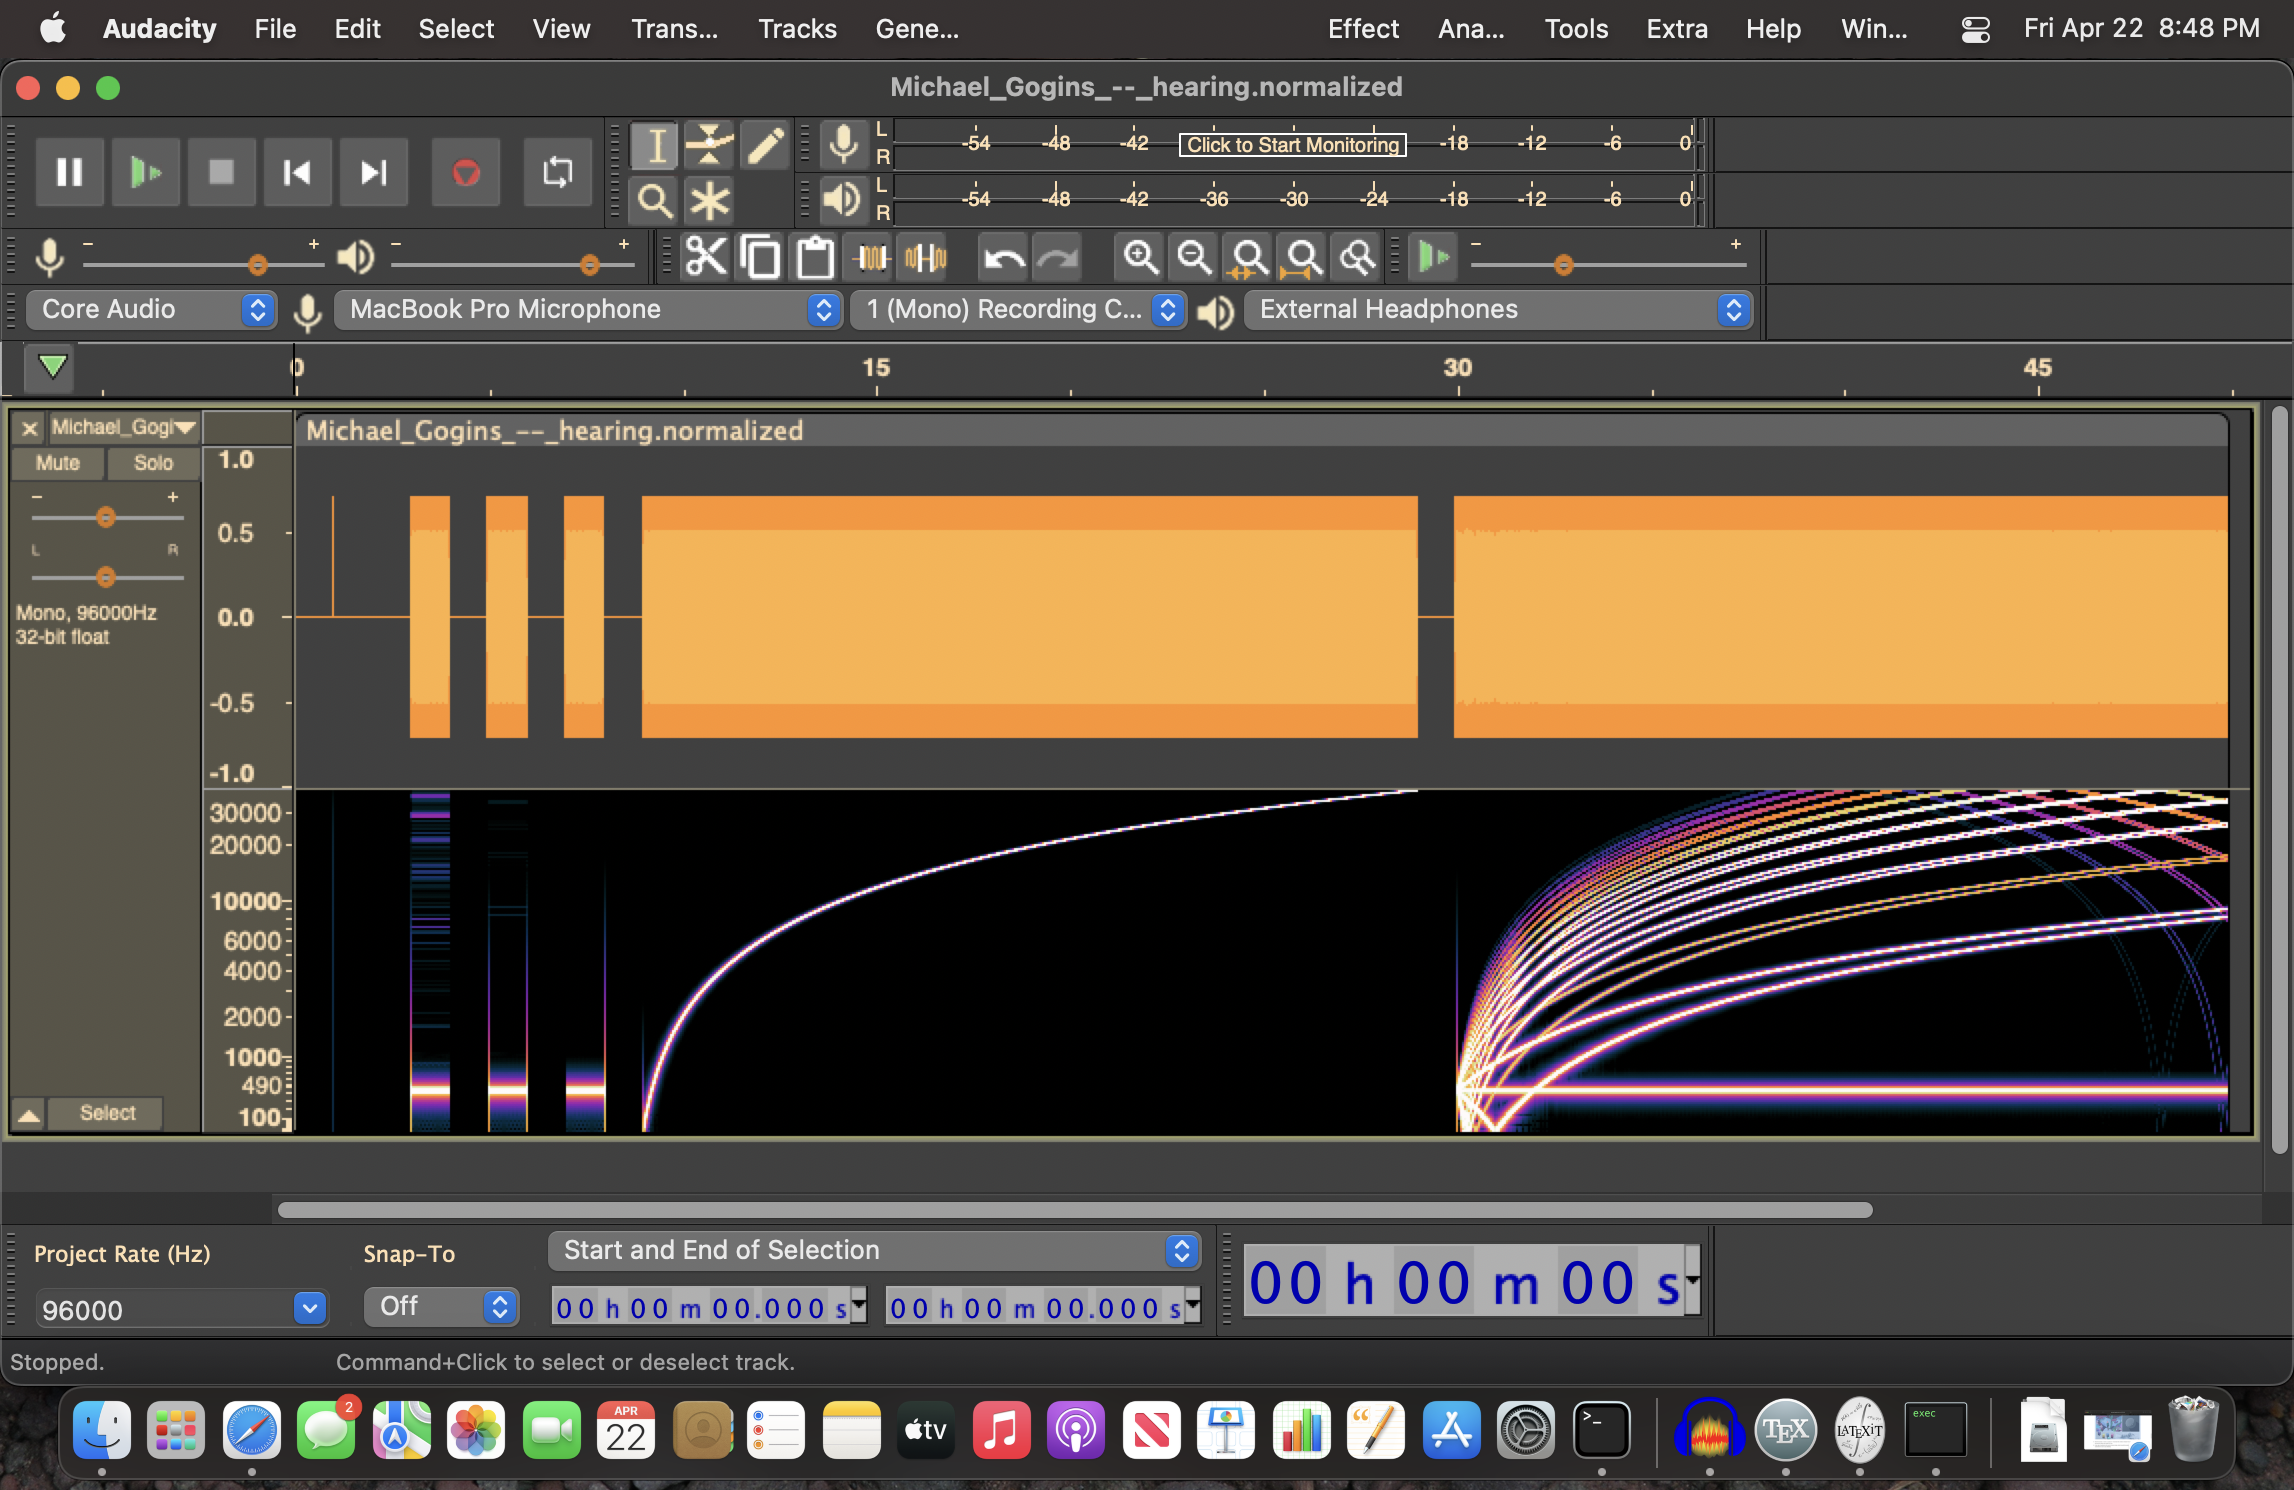
\includegraphics[height = 0.66\textwidth]{hearing}}
\end{figure}
\end{frame}

\begin{frame}{Hearing electroacoustically}
\begin{itemize}
\item The initial spike shows that a 1 sample click contains all frequencies up to the Nyquist frequency.
\item The next three columns show the effects of increasing wave table size on noise.
\item The first arc shows a frequency sweep from 0 up to 40 KHz, though the sampling rate is 48 KHz.
\item What can you really hear? Where does your ability to hear high frequencies end? Use good headphones.
\item As for me, I can't hear anything past about 12 KHz.
\end{itemize}
\end{frame}

\begin{frame}{Hearing electroacoustically}
\begin{itemize}
\item The second set of arcs shows aliasing of an FM tone as the frequency of the modulating signal increases. 
Note the \emph{negative} aliasing, which reflects off frequency 0.
\item After the arcs, there is a single cosine grain .01 seconds long.
\item Then there is a note with a non-releasing envelope, and the same note with a releasing envelope.
\item Finally, there are bands where a source sound is convolved with an increasingly longer impulse sound.
\end{itemize}
\end{frame}

\begin{frame}{Hearing electroacoustically}
\begin{itemize}
\item In Audacity, zoom in on the single short grain.
\item Change the spectrogram window to the smallest size.
\item Time is well-resolved, but \emph{all} frequencies are shown in the spectrogram, i.e. there is \emph{no} frequency resolution.
\item Change the spectrogram window to the largest size.
\item Frequency is now well-resolved, but the energy is smeared out \emph{well} before and after the grain.
\item This shows the time/frequency uncertainty that exists in all convolution and spectral processing.
\item The minimal area of resolved energy is called the Gabor logon. It can get taller or wider, but its area is constant.
\end{itemize}
\end{frame}

\begin{frame}{Hearing electroacoustically}
\begin{itemize}
\item In Audacity, zoom in on the two notes after the grain.
\item The first note uses a long exponential decay with no release, so it just cuts off at the end of the note.
\item This causes a discontinuity in the waveform, which is the same as noise in the frequency domain. The spectrogram shows this as  energy spread out in the vertical dimension.
\item The second note is exactly the same, but using the releasing form of the envelope.
\item Clicks are a bedeviling artifact of digital audio, because avoiding discontinuities in digital signals is hard.
\item Natural sounds don't tend to have such discontinuities, as physical energy takes time to build up or to release.
\item Always use a releasing envelope or a de-clicking envelope.
\end{itemize}
\end{frame}

\begin{frame}{Hearing electroacoustically}
\begin{itemize}
\item Finally, there are four bands at the end of the soundfile.
\begin{enumerate}
\item An original recording of junk noises from my apartment.
\item Junk convolved with a .01 second bell sound. It's subtle, a bit of ringing on the final note.
\item Junk convolved with a .1 second bell sound. The convolution can be heard on all sounds. There is a kind of ringing from the impulse.
\item Junk convolved with a 1 second bell sound. The original sounds are obscured by the ringing of the long impulse.
\end{enumerate}
\item The ringing is an artifact \emph{in some contexts}, I call it "convolution smear."
\item What is true of convolution is true of every linear time-invariant system. A positive frequency in the impulse produces ringing, a negative frequency causes notching. Maybe you \emph{want} it, maybe not, but \emph{notice} it.
\end{itemize}
\end{frame}

\begin{frame}{Coding for high-resolution audio}
\begin{itemize}
\item Many of Csound's opcodes, man pages, and examples are old, and
prioritize memory and run time over audio quality.
\item \textit{Today, \textbf{prioritize audio quality} in all cases}.
\item Use a sample rate of 48,000 or even 96,000 frames per second with
\texttt{ksmps = 100} or even \texttt{ksmps = 1}.
\item Use the double-precision version of Csound (now default).
\item Render to floating-point soundfiles for high dynamic range.
\item Use table sizes of at least 65,537 for lower noise.
\item Use \textit{audio-rate} envelopes to prevent zipper noise.
\item Use releasing or de-clicking envelopes on all final outputs.
\item Use the \textit{latest versions} of opcodes.
\item Used like this, Csound has unsurpassed audio quality.
\end{itemize}
\end{frame}

\begin{frame}{Exercise: Coding for high-resolution audio}
\begin{example}
Change to the \texttt{exercises/resolution} directory in your workshop directory.
\begin{itemize}
\item Execute \texttt{~/playpen.py csd-play xanadu.csd}, listen on headphones, and examine the spectrogram in Audacity.
\item Execute \texttt{~/playpen.py csd-play xanadu-high-resolution.csd} the high-resolution version, listen on headphones, and examine the spectrogram in Audacity.
\end{itemize}
\end{example}
\end{frame}

\begin{frame}{Original Xanadu}
\begin{figure}
\centerline{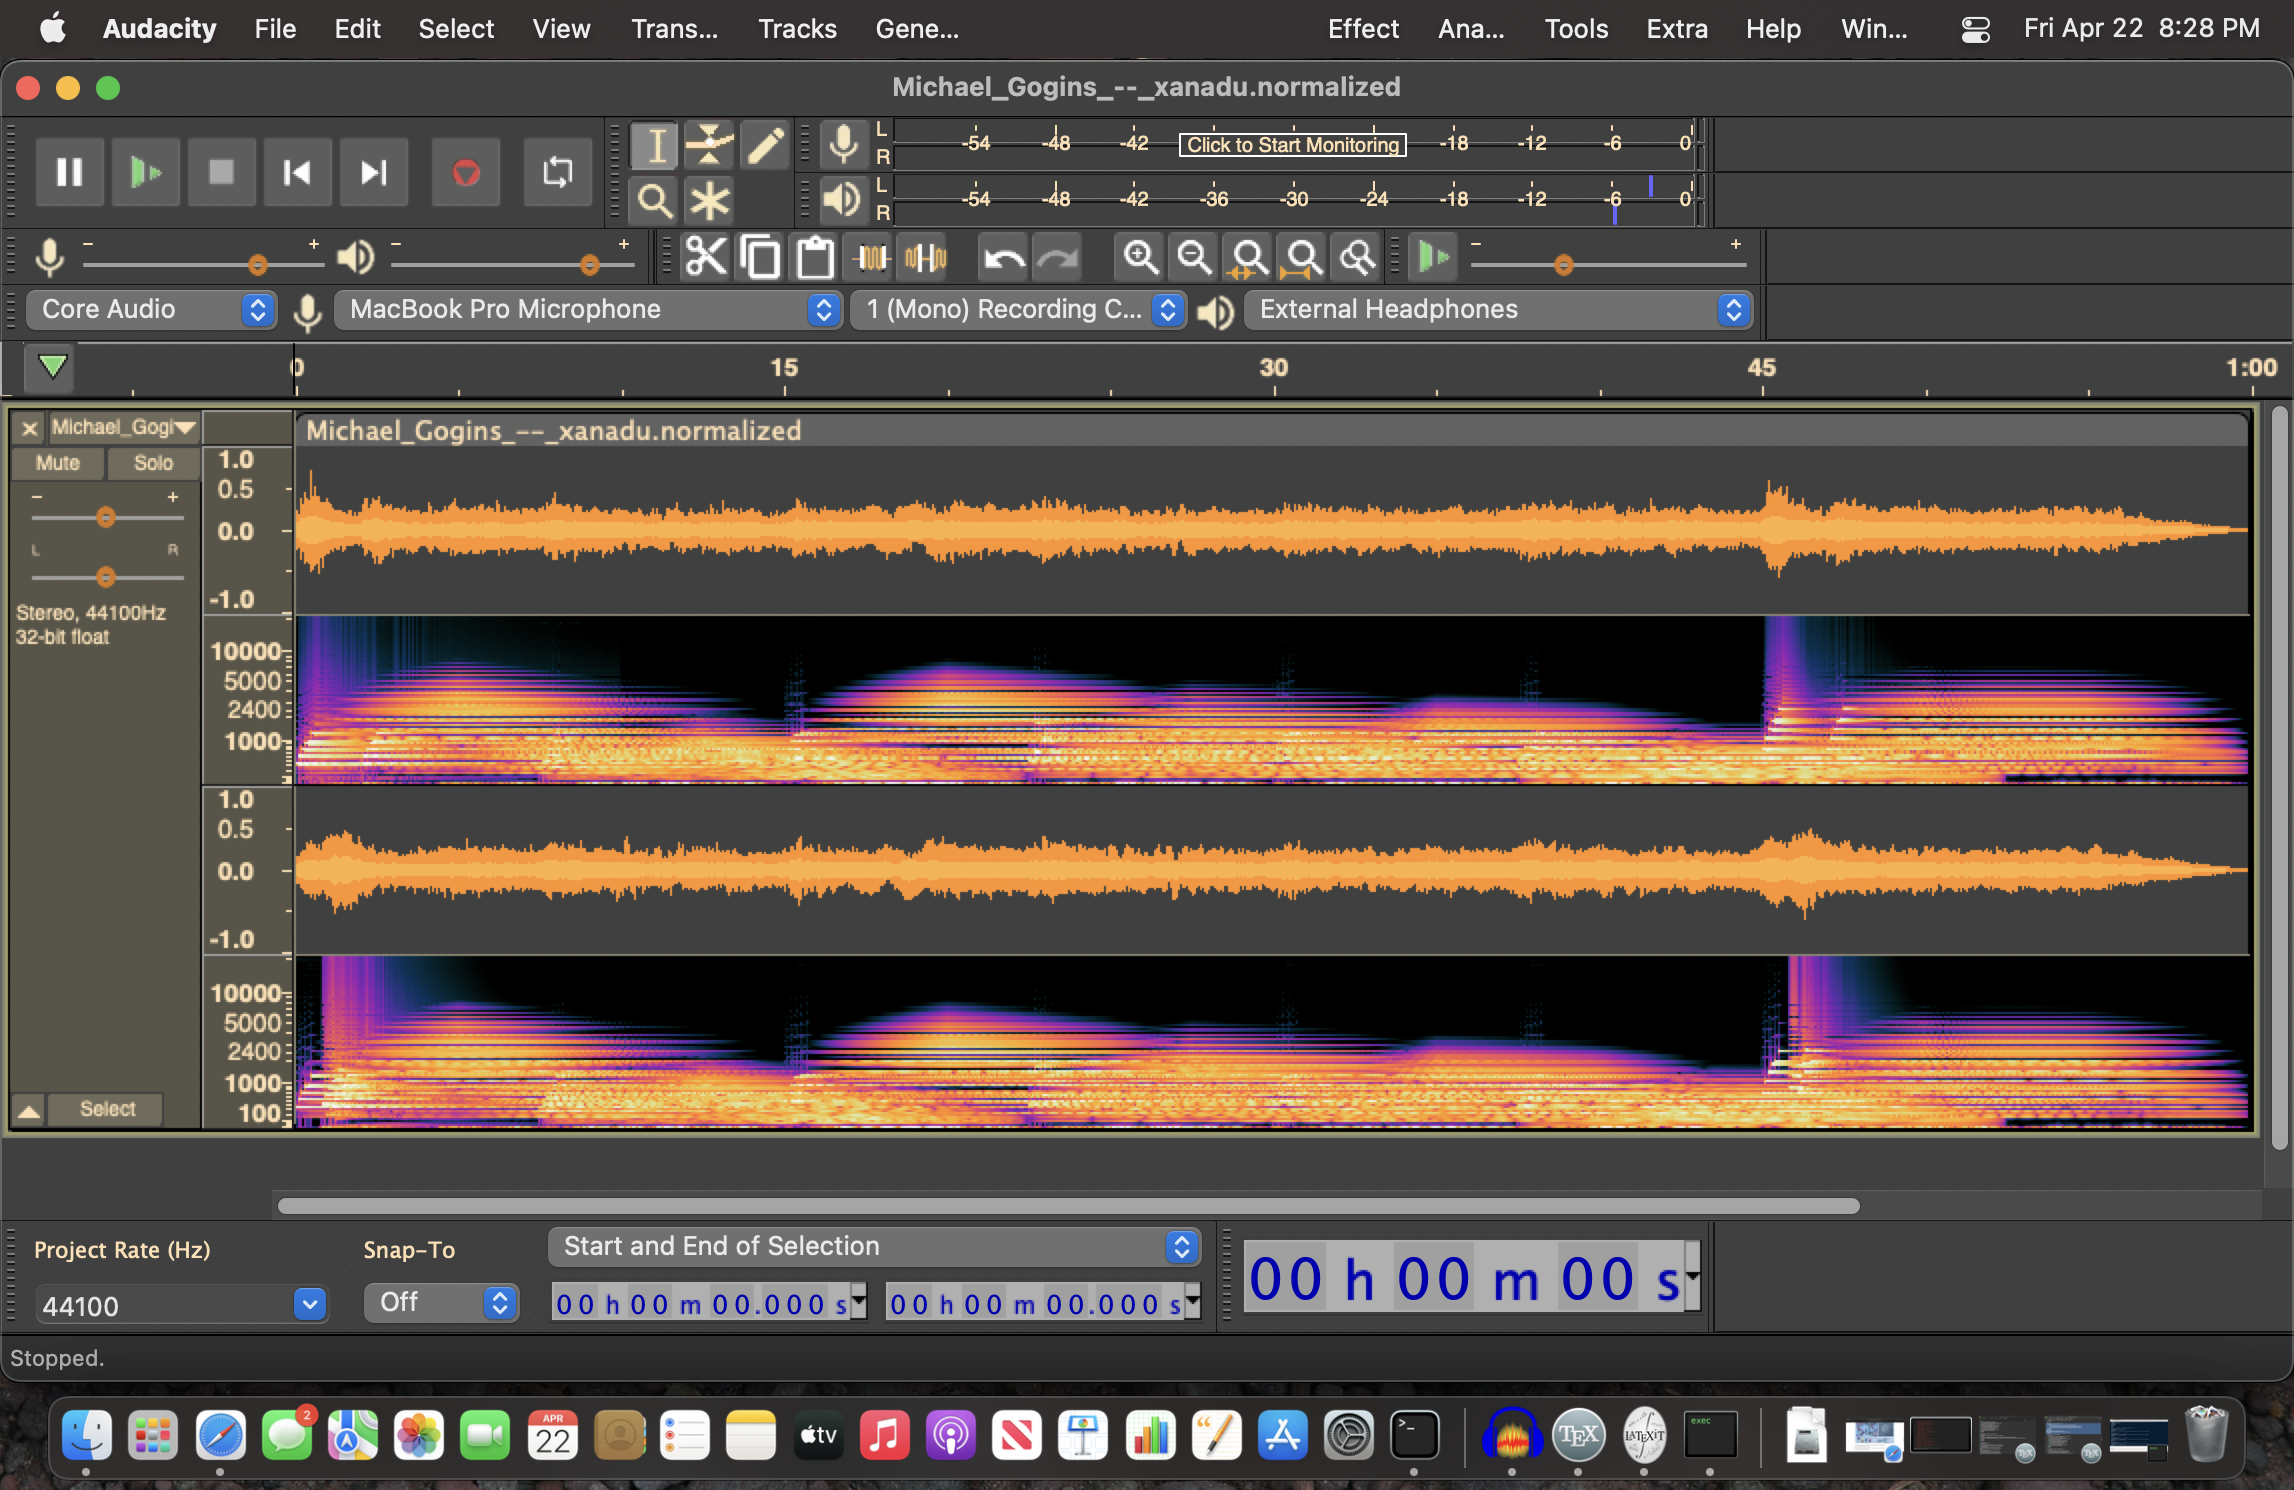
\includegraphics[height = 0.66\textwidth]{xanadu}}
\end{figure}
\end{frame}

\begin{frame}{High-Resolution Xanadu}
\begin{figure}
\centerline{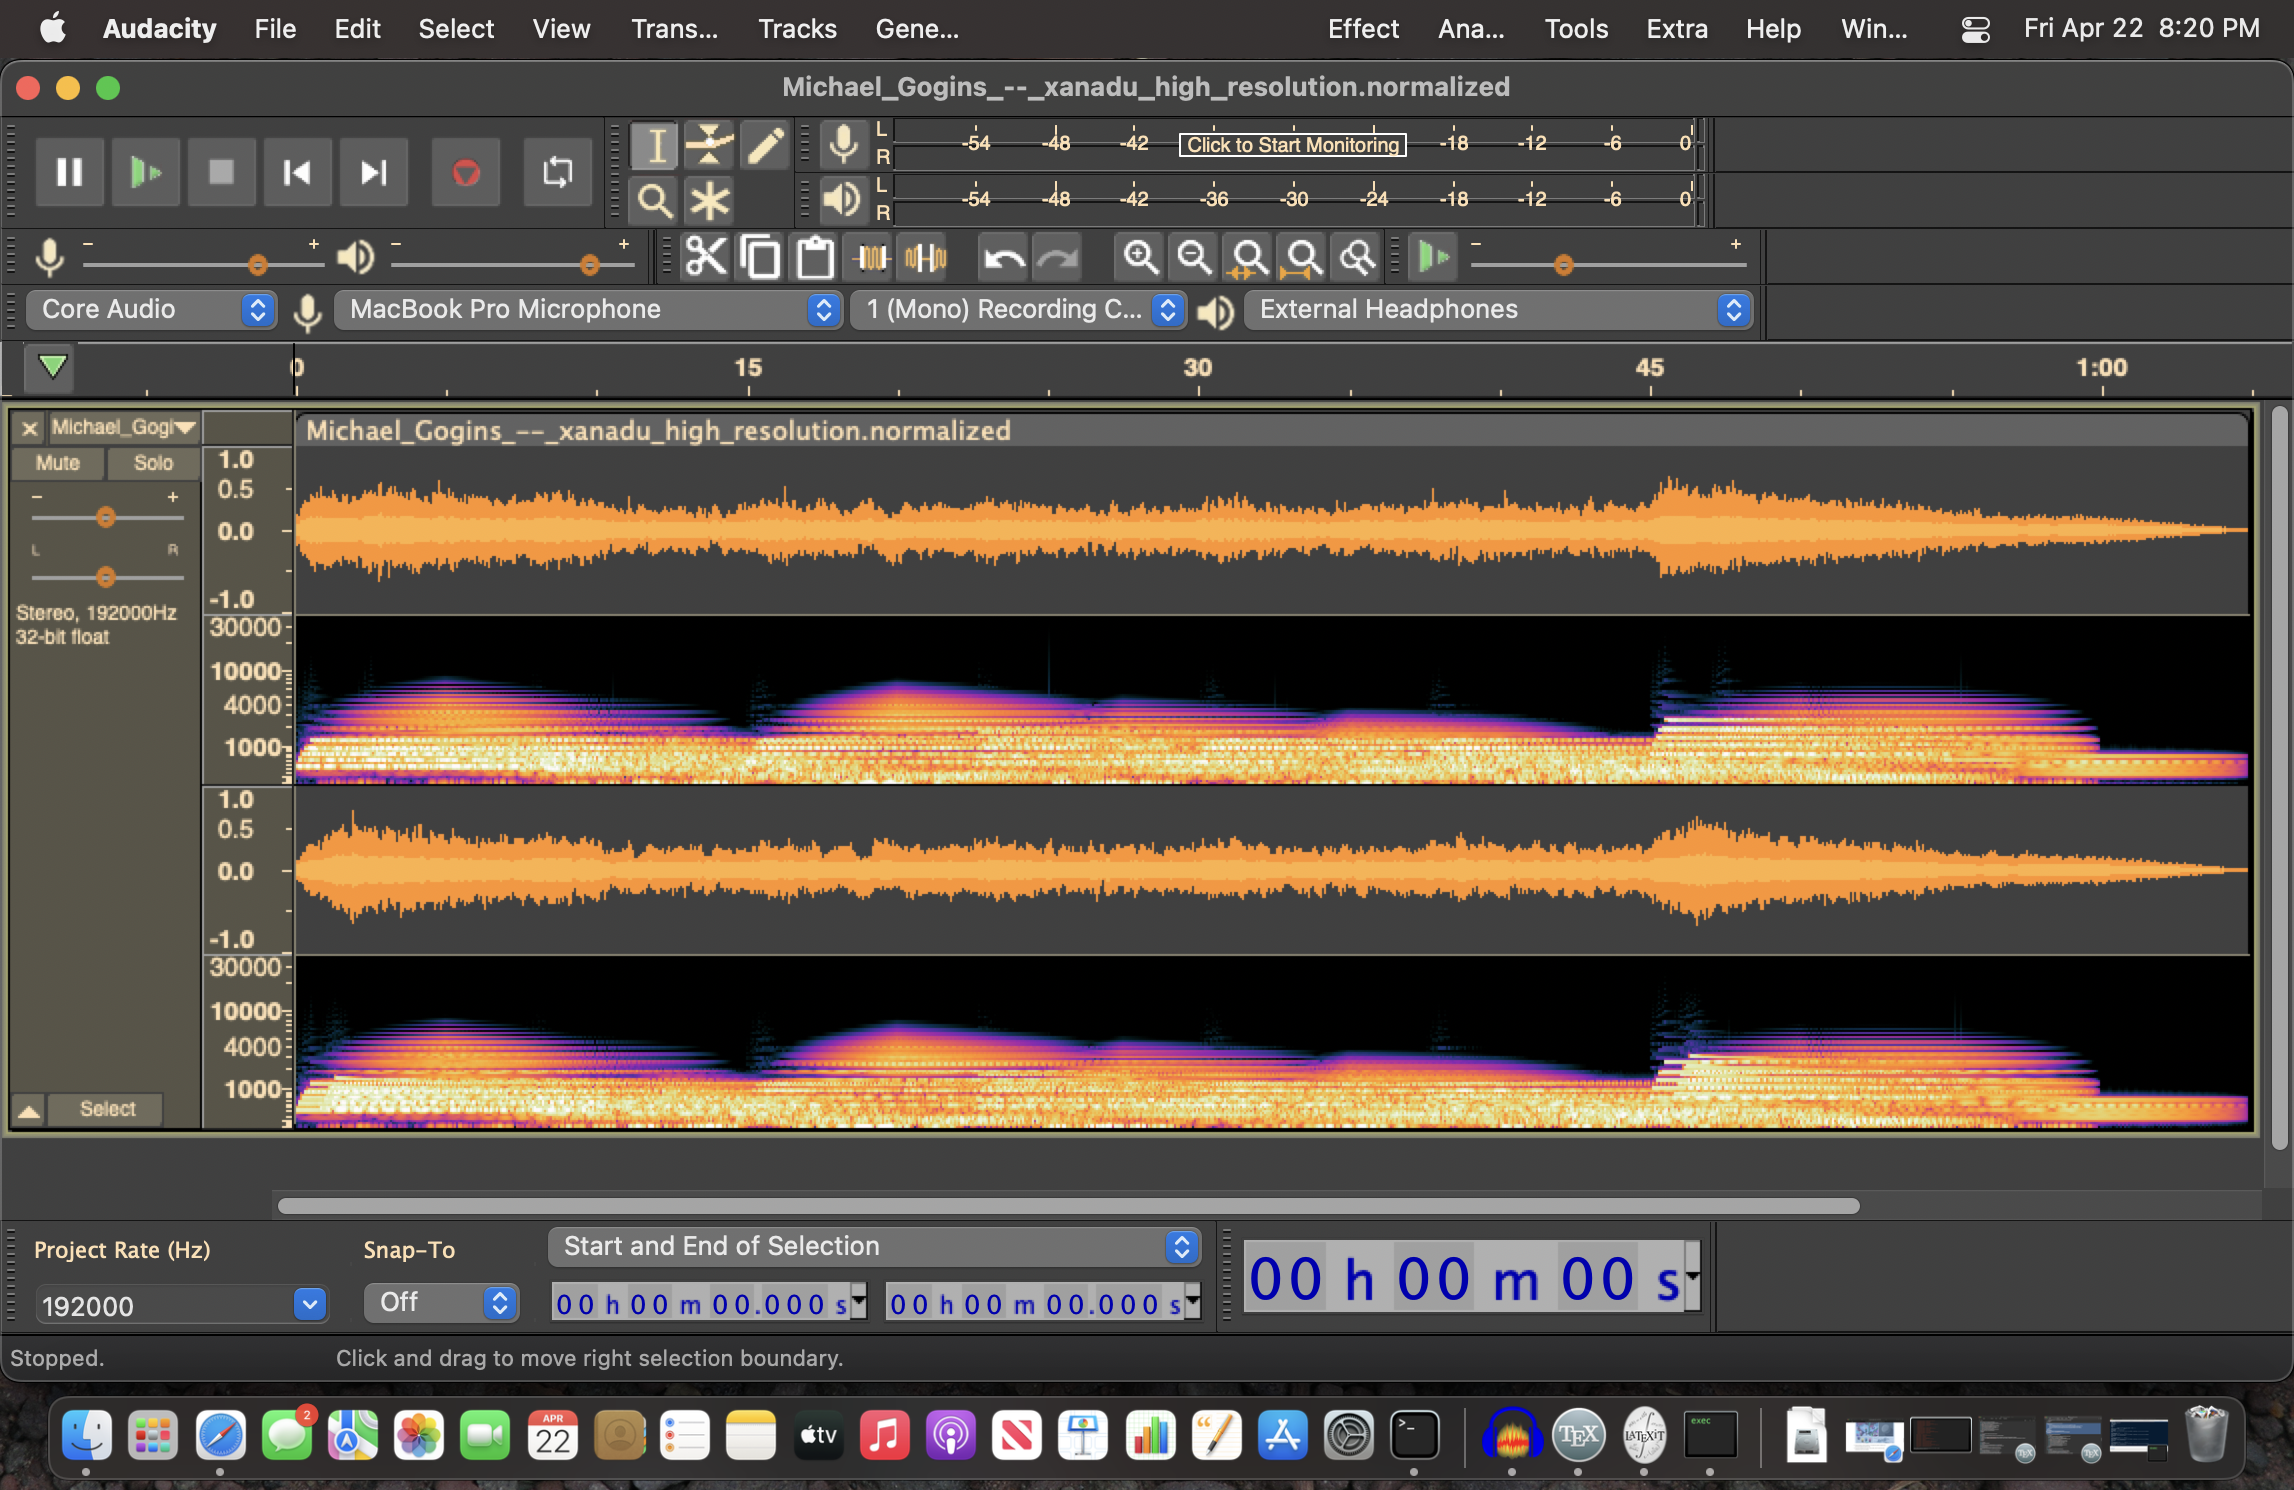
\includegraphics[height = 0.66\textwidth]{xanadu-high-resolution}}
\end{figure}
\end{frame}

\begin{frame}{Useful opcodes}
Exercises for some of these follow.
\begin{itemize}
\item \texttt{transegr}: most flexible envelope generator.
\item \texttt{ftgen}: move function tables from score to orchestra.
\item \texttt{poscil}, \texttt{poscil3}: most precise oscillators.
\item \texttt{crosspm}, \texttt{crosspmi}: phase modulation/frequency modulation.
\item Fluidsynth opcodes for SoundFonts (plugin).
\item Opcodes for Faust DSP language (plugin).
\item \texttt{diskin2}: flexible soundfile input.
\item \texttt{deltapi}: building block for physical models.
\item \texttt{PVS} opcodes: toolkit for time/frequency operations.
\end{itemize}
\end{frame}

\begin{frame}{transegr}
\begin{example}
Change to the \texttt{exercises/opcodes} directory of your workshop directory.
\begin{itemize}
\item Execute \texttt{$\sim$/playpen.py csd-play transegr.csd} and view the soundfile in Audacity.
\end{itemize}
\end{example}
\begin{itemize}
\item Observe that an exponent of 0 creates linear segments, a negative exponent creates concave segments.
\item See how the \texttt{r} (release) suffix handles termination of notes without clicking.
\item No need for any other envelope opcode.
\end{itemize}
\end{frame}

\begin{frame}{deltapi}
\begin{example}
Change to the \texttt{exercises/opcodes} directory of your workshop directory.
\begin{itemize}
\item Execute \texttt{$\sim$/playpen.py csd-play livingston-guitar.csd} and view the soundfile in Audacity.
\item Read the code to see how double delay lines with filters model reflecting waves in strings.
\end{itemize}
\end{example}
\end{frame}

\begin{frame}{FluidSynth opcodes}
\begin{example}
Change to the \texttt{exercises/fluid} directory of your workshop directory.
\begin{itemize}
\item TODO
\end{itemize}
\end{example}
\end{frame}

\begin{frame}{Faust opcodes}
\begin{example}
Change to the \texttt{exercises/faust} directory of your workshop directory.
\begin{itemize}
\item TODO
\end{itemize}
\end{example}
\end{frame}

\begin{frame}{PVS opcodes}
\begin{example}
Change to the \texttt{exercises/pvs} directory of your workshop directory.
\begin{itemize}
\item TODO
\end{itemize}
\end{example}
\end{frame}


\section{Coding for Csound}
\begin{frame}{Software design}
\begin{itemize}
\item \textbf{Encapsulation} Hide implementations in \textit{modules} that
expose only inputs and outputs. Define modules with \texttt{instr} (classes) and
\texttt{opcode} (functions).
\item \textbf{Abstraction} Define abstract interfaces for instruments or
UDOs that perform similar functions; e.g. different synths use the same
pfields.
\item \textbf{Normalization} Use \textit{musical} units: MIDI key not
Hz, MIDI velocity not amplitude.
\item \textbf{Signal Flow} Signals flow from input devices through
opcodes to instruments; from opcode to opcode through variables; from
instruments through opcodes to output devices. Processing is first by
instrument number, then by order of definition. Signals also flow through
control channels and global variables.
\end{itemize}
\end{frame}

\begin{frame}{Modular design}
\begin{itemize}
\item Using naming conventions to simulate namespaces.
\item Normalize pfields and variables.
\item Associate global function tables with modules.
\item Associate global control variables with modules, and use
\texttt{chnexport} to export these variables as control channels.
\item Define signal flow in the orchestra header, \textit{not} inside modules.
\item Use the MIDI interop command line options so the same instruments work for both MIDI and scores.
\end{itemize}
\end{frame}

\begin{frame}{Modules in Csound}
\begin{example}
Change to the \texttt{exercises/coding} directory of your workshop directory.
\begin{itemize}
\item Execute \texttt{$\sim$/playpen.py csd-play modules.csd} and view the soundfile in Audacity.
\end{itemize}
Read the code...
\begin{itemize}
\item Function tables are created as global variables associated with the instrument definition.
\item To that end, namespaces are implemented using prefixes to names.
\item Note "natural" units (MIDI key, MIDI velocity) in the score.
\item Note instruments can be re-ordered, added, removed; all connections are made in the orc header.
\end{itemize}
\end{example}
\end{frame}

\section{Plugins}

\begin{frame}{Plugins}
\begin{itemize}
\item Csound has its own plugin format, not only for plugin opcodes, but also for plugin function table generators.
\item Csound also has opcodes that can load non-Csound plugins:
\begin{itemize}
\item VST2 plugins, now deprecated by Steinberg (freeware from me).
\item VST3 plugins, now free software (on GitHub from me).
\item The Jack Audio Connection Kit (JACK) can be considered a kind of plugin protocol. Csound supports JACK both as an input/output driver, and with the Jacko plugins from me.
\end{itemize}
\item Plugins are available from \emph{many} sources. The largest number are VST plugins.
\end{itemize}
\end{frame}

\begin{frame}{Sources of Csound plugins}
\begin{itemize}
\item Csound external plugins repository.
\item The Risset package manager for Csound plugin opcodes.
\item \texttt{vst4cs} opcodes. Not discussed here as VST2 is now deprecated by Steinberg.
\item \texttt{csound-vst3-opcodes}.
\end{itemize}
\end{frame}

\begin{frame}{External Csound plugins repository}
\begin{itemize}
\item This contains opcodes former in Csound's GitHub repository that have external dependencies, and so were moved to their own repository.
\item These currently need to be built from source code, which is not difficult if you can program.
\item Go to \url{https://github.com/csound/plugins} to see what's currently available.
\end{itemize}
\end{frame}

\begin{frame}{csound-vst3-opcodes}
This assumes you have installed \texttt{csound-vst3-opcodes}, or built them from sources.
\begin{example}
Change to the \texttt{exercises/plugins} directory of your workshop directory.
\begin{itemize}
\item Execute \texttt{$\sim$/playpen.py csd-play vst3-opcodes-minimal.csd} and view the soundfile in Audacity.
\end{itemize}
\end{example}
\end{frame}

\begin{frame}{Opcodes in Risset}
\begin{example}
Change to the \texttt{exercises/plugins} directory of your workshop directory.
\begin{itemize}
\item Execute \texttt{python3 -m risset list} to view all plugins in the repository.
\item Execute \texttt{python3 -m risset show beosc} to view details on the band-limited+noise  oscillator opcodes.
\end{itemize}
\end{example}
\end{frame}

\section{Other languages}
\begin{frame}{Csound and other languages}
\begin{itemize}
%% The examples all have to use the same simple orchestra and simple algorithmic score generator.
\item The following exercises all implement the same Csound piece, for purposes of comparison.
\item Embed Csound in Python with \texttt{ctcsound}.
\item Embed C++ in Csound with \texttt{csound-cxx-opcodes}.
\item Embed Csound in C++ with \texttt{csound\_threaded.hpp}.
\item There are many other language bindings for Csound....
\end{itemize}
\end{frame}

\begin{frame}{Csound in Python}
\begin{example}
Change to the \texttt{exercises/languages} directory of your workshop directory.
\begin{itemize}
\item Execute \texttt{python3 csound-in-python.py}
\item Open \texttt{csound-in-python.py} in Audacity to see and hear the soundfile.
\end{itemize}
\end{example}
\end{frame}

\begin{frame}{C++ in Csound}
\begin{example}
Change to the \texttt{exercises/languages} directory of your workshop directory.
\begin{itemize}
\item Execute \texttt{csound cplusplus-in-csound.csd} to render the piece.
\item Open \texttt{cplusplus-in-csound.wav} in Audacity to see and hear the soundfile.
\end{itemize}
\end{example}
\end{frame}

\begin{frame}{Csound in C++}
\begin{example}
Change to the \texttt{exercises/languages} directory of your workshop directory.
\begin{itemize}
\item Execute \texttt{$\sim$/playpen.py cpp-app csound-in-cplusplus.cpp} to compile the piece.
\item Execute \texttt{./csound-in-cplusplus} to run the piece.
\item Execute \texttt{open csound-in-cplusplus.wav} to view and hear the soundfile.
\end{itemize}
\end{example}
\end{frame}

\end{document}
